\section{Preliminaries}
\subsection{AdS/CFT correspondence}
%
%
Among the most exciting breakthroughs in theoretical physics in the last decades there certainly is the famous conjecture made by Maldacena in 1997 \cite{maldacena1}, now widely known as $AdS/CFT$ correspondence which attracted many scientists to contribute their work to this field of study.\\
What makes this conjecture so promising is that it relates a quantum field theory (QFT) of gauge fields in flat spacetime with a string theory. The latter one is also a promising candidate for a theory of quantum gravity. Unifying gravity with the other fundamental forces condensed in the Standard Model would be one of the next big milestones in physics. By studying the predictions of the $AdS/CFT$ correspondence scientists hope to get one step closer to this fundamental aim. 
%The $AdS/CFT$ correspondence is some sort of strong-weak coupling duality. It can relate a strong coupled field theory to its dual, a weakly curved gravity theory. 
The conjecture links two theories, very different in their physical content and interpretation, stating that they are mathematically equivalent.
The $AdS$ part refers to a gravity theory on asymptotically Anti-de Sitter spacetime,  $CFT$ stands for conformal field theory. In its primary form \cite{Ammon:2015wua}, the correspondence states that \\[0.2cm]
%
%
%
\begin{tcolorbox}[colback=white!95!black, colframe=white!90!black]
\begin{center}
\textbf{Type IIB superstring theory} \\
with string length $l_{\rm s}=\sqrt{\alpha'}$ and coupling constant $g_{\rm s}$ on $AdS_{5}\times S^{5}$ with radius of curvature $R$ and $N$ units of $F_{(5)}$ flux on $S^{5}$
\end{center}
\end{tcolorbox}
%
\begin{equation*}
\uparrow \qquad \textit{is dynamically equivalent to} \qquad \downarrow
\end{equation*}\hspace{1mm}
%
%
\begin{tcolorbox}[colback=white!95!black, colframe=white!90!black]
\begin{center}
\textbf{$\mathcalbf{N}\bm{=}\mathbf{4}$ Super \names{Yang-Mills} theory}\\
with gauge group $SU(N)$ and \names{Yang-Mills} coupling constant $g_{\rm YM}$.
\end{center}
\end{tcolorbox}
%
%
\noindent By the conjecture the free parameters on the field theory side $g_{\rm YM}$ and $N$ are mapped to the free parameters $g_{\rm s}$ and $R/\sqrt{\alpha'}$ on the string theory side by
%
%
\begin{tcolorbox}[colback=white!95!black, colframe=white!90!black]
\begin{equation}
\frac{4\pi \lambda}{N} =  g_{\rm s} \quad {\rm and} \quad \lambda \equiv g_{\rm YM}^{2}N = \frac{R^{4}}{\alpha'^{2}}\,.
\end{equation}
\end{tcolorbox}
%
%
In the second equation we defined the \names{'t Hooft} coupling $\lambda$. String theory is yet best understood in the perturbative regime, therefore it is convenient to restrict the coupling on the string theory side to $g_{\rm s}\ll 1$, while keeping $R/\sqrt{\alpha'}$ constant. The $AdS$ side reduces then, at leading order in $g_{\rm s}$ to classical string theory. The quantity $R^{2}/\alpha'$ is kept constant.  Also the coupling on the $CFT$ side is conveniently taken to be small, $g_{\rm YM} \ll 1$, while $g_{\rm YM}^{2}N$ is kept finite. We therefore have to take the large $N$ limit $N \to \infty$ with $\lambda$ fixed, which is also known as the \names{'t Hooft} limit. This corresponds to the planar limit of the gauge theory. We are then left with $\lambda$ as the free parameter of the $AdS/CFT$ system. In the limit of large $\lambda$, and therefore $\alpha'/R^{2}\to 0$ or large curvature $R$, the string does not feel the effect of the interaction created by the (now weakly curved) background. So for large $\lambda$ one is in the perturbative regime of string theory, whereas the gauge theory side is perturbatively accessible for $\lambda \ll 1$.
%
% We want to investigate the $AdS/CFT$ correspondence numerically from the string theory side and therefore know solutions for large $\lambda$ from perturbation theory. Now we can make use of the previously stated relation by going to smaller couplings where we leave the perturbative regime of string theory but enter the selfsame for the gauge theory side. This means that when we do numerical simulations for small couplings in string theory, then we still might be able to compare these results with predicted solutions of the perturbative regime of gauge theory. 
%
The fact that the perturbative (accessible) regimes of both models do not overlap - which is referred to as a weak-strong coupling duality - is on one side very fascinating, as it allows the exploration of the strong coupling regime of a theory via the study of the much simpler dual model.
On the other side, it makes highly non-trivial any dynamical and direct check of the $AdS/CFT$ correspondence. In this thesis we address the problem of realizing such direct checks numerically within the string worldsheet model. In the latter, we control the large $\lambda$ regime where we know analytical solutions. The lattice, numerical approach will allow us to leave the perturbative regime and go to smaller $\lambda$, where 
comparison with the solutions of  perturbative gauge theory is - once the difficulties peculiar to this approach are tamed - possible. 
In fact, in the case under study we can also attempt a comparison between string and gauge theory at finite values of $\lambda$, where together with the $AdS/CFT$ hypothesis another powerful conjecture - the integrability of the underlying system -  is available with its predictions.
%
%
%
%
%
%
% - - - - - - - - - - - - - - - - - - - - - - - - - - - - - - - 
%               WILSON LOOPS
% - - - - - - - - - - -- - - - - - - - - - - - - -- - - - - - - 
%
%
\subsection{Wilson loops}
%
An important class of observables in gauge theories are non-local gauge invariant operators called \names{Wilson} loops. These operators are evaluated along a given closed path $\mathcal{C}$. For specific cusped paths one can (in a certain limit) extract a function, called cusp anomaly, from the \names{Wilson} loop. According to $AdS/CFT$ the minimal surface of a string ending on a certain path gives (in a certain regime) the value of the corresponding \names{Wilson} loop. We therefore can extract information about the cusp anomaly function also from the string theory side. To make this remark more explicit, we first want to review some more details about \names{Wilson} loops.\\
For pure \names{Yang-Mills} theory with the gauge group $SU(N)$ the \names{Wilson} loop $W[\mathcal{C}]$ is a path-ordered exponential of a gauge field $A_{\mu}$ along a closed contour $\mathcal{C}$, which in the fundamental representation is defined by
%
%
\begin{equation}
W[\mathcal{C}] = \frac{1}{N}{\rm Tr} \left( \mathcal{P} \exp \left[ i \oint\limits_{\mathcal{C}} \dd x^{\mu}A_{\mu} \right] \right).
\end{equation}
%
%
Here the trace is over the fundamental representation of the gauge group and $\mathcal{P}$ is the path ordering operator. If we choose to parametrise the curve $\mathcal{C}$ as $x^{\mu}(s)$ with $s \in [0,1]$, we can write the exponent as
\begin{equation}
 i \oint\limits_{\mathcal{C}} \dd x^{\mu}A_{\mu} =  i \int\limits_{0}^{1} \dd s \frac{\dd x^{\mu}}{\dd s} A_{\mu}\left(x\left(s \right)\right)\,.
\end{equation}
Actually we have $A_{\mu}=A_{\mu}^{a}T_{a}$, where $T_{a}$ is a generator of the \names{Lie} algebra $\mathfrak{su}(N)$ of the gauge group and therefore different fields $A_{\mu}$ do not commute in general. To avoid appearing ambiguities in the ordering of fields due to a \names{Taylor} expansion of the exponential, the operator $\mathcal{P}$ is ordering them in the following sense
\begin{equation}
\mathcal{P}\left( A\left(x\left(s_{1}\right)\right) A\left(x\left(s_{2}\right)\right) \right)
= \left\lbrace \begin{matrix}
A\left(x\left(s_{1}\right)\right) A\left(x\left(s_{2}\right)\right) \quad {\rm for} \; s_{1}>s_{2},  \\ 
A\left(x\left(s_{2}\right)\right) A\left(x\left(s_{1}\right)\right) \quad {\rm for} \; s_{2}>s_{1}.
\end{matrix} \right.
\end{equation}
%
%
%
\subsection{Wilson loops in $AdS/CFT$}
Since the action of four-dimensional $\mathcal{N}=4$ SYM can be derived via dimensional reduction from $\mathcal{N}=1$ SYM in ten dimensions \cite{BRINK197777} one can construct a \names{Wilson} loop there, starting from its definition in the ten dimensional gauge theory. By using the field theory content of the four-dimensional theory $A_{\mu}$ and $x^{\mu}$ and six additional scalar fields of $SU(N)$ the so called \names{Maldacena-Wilson} loop proposed in \cite{maldacena2} can be written as
%
%
\begin{equation}
\mathcal{W}[\mathcal{C}] = \frac{1}{N}{\rm Tr}\mathcal{P} \exp \left( \int\limits_{\mathcal{C}} \dd s \left( i A_{\mu}(x)\dot{x}^{\mu} +
\vert \dot{x}\vert \phi_{I}(x) n^{I} \right) \right) \,.
\end{equation}
%
%
Here $I=1,\ldots,6$ and $n^{I}$ might be considered coordinates in $S^{5}$, satisfying $\delta_{IK}n^{I}n^{K}=1$. The curve described by $n^{I}(s)$ in the five-sphere must not necessarily be closed. \\
%
%
In the context of $AdS/CFT$ the \names{Maldacena-Wilson} loop also has a corresponding string theory description, which was first proposed in \cite{maldacena2}. Thus the expectation value of the \names{Maldacena-Wilson} loop operator is given by a string partition function
%
%
\begin{equation}
\langle \mathcal{W}[\mathcal{C}]\rangle = Z_{\rm string}[\mathcal{C}],
\label{W_Z}
\end{equation}
%
%
which is a path integral obeying suitable boundary conditions
%
%
\begin{equation}
Z_{\rm string}[\mathcal{C}] = \int\limits_{\del X^{\mu}=\mathcal{C}} \mathcal{D}X^{M}\, \mathcal{D}h_{\alpha\beta}\, \exp \left(-S_{\rm string}\left( X,h \right) \right)\,.
\label{Z_string}
\end{equation}
%
%
Here $S_{\rm string}$ is the action of the fundamental string in $AdS_{5}\times S^{5}$, $h_{\alpha\beta}$ a 2d metric and ${X^{M}=(X^{\mu},X^{3+I})}$ ${(M=0,\ldots,9;\, \mu=0,\ldots,3; \; I=1,\ldots,6)}$ are the embedding functions in the string target space, depending on the worldsheet coordinates $(\tau,\sigma)\in \Sigma$ where $\Sigma$ representing a map of the string worldsheet. By defining $\widetilde{X}^{I}=X^{3+I}$ and therefore $X^{M}=(X^{\mu},\widetilde{X}^{I})$ the partition function (\ref{Z_string}) needs to meet the following boundary conditions
%
%
\begin{equation}
\left. X^{\mu} \right\vert_{\del \Sigma} = x^{\mu}(s) \,,\quad   \left.\frac{\widetilde{X}^{I}}{\vert \widetilde{X}^{I}\vert} \right\vert_{\del \Sigma} = n^{I}(s) \,, \quad   \left. \vert \widetilde{X}^{I} \vert \right\vert_{\del \Sigma} = 0\,,
\end{equation}
%
%
where $x^{\mu}(s)$ parametrises the curve $\mathcal{C}$. One can show that the conformal boundary of $AdS_{5}\times S^{5}$ is 4d \names{Minkowski} space\footnote{At the conformal boundary the five-sphere appears to have zero extent. See (\ref{AdS5}) for details on the conformal mapping of $AdS_{5}$ to flat 4d \names{Minkowski} space.}. Therefore one can say that the embedding of the string worldsheet is bounded by the curve $\mathcal{C}$, see \autoref{Wilson_worldsheet}. In the large \names{'t Hooft} coupling limit $\lambda \gg 1$, the path integral (\ref{Z_string}) can be evaluated with a saddle point approximation and results in the exponential of a minimal surface $\mathcal{A}_{\rm min}(\mathcal{C})$ bounded by $\mathcal{C}$
%
%
\begin{equation}
\langle \mathcal{W}[\mathcal{C}]\rangle \simeq \exp \left( \frac{\sqrt{\lambda}}{2\pi} \mathcal{A}_{\rm min}(\mathcal{C}) \right).
\end{equation}
%
%
\begin{figure}
\begin{center}
\begin{tikzpicture}
\node[anchor=south west,inner sep=0] (image) at (0,0) {\includegraphics[width=0.35\textwidth]{Wilson_worldsheet.png}};
\begin{scope}[x={(image.south east)},y={(image.north west)}]
\node [anchor=west] at (0.088,0.4) {$\mathcal{C}$};
\node [anchor=west] at (0.8,0.6) {$\widetilde{\Sigma}$};
\node [anchor=west] at (0.95,0.1) {$z$};
%\draw[help lines,xstep=.1,ystep=.1] (0,0) grid (1,1);
%\foreach \x in {0,1,...,9} { \node [anchor=north] at (\x/10,0) {0.\x}; }
%\foreach \y in {0,1,...,9} { \node [anchor=east] at (0,\y/10) {0.\y}; }
\end{scope}
\end{tikzpicture}
\caption{The embedding of the string worldsheet $\widetilde{\Sigma}$ in $AdS_{5}\times S^{5}$ is bounded by the contour $\mathcal{C}$ as $z$ approaches zero.\label{Wilson_worldsheet}}
\end{center}
\end{figure}
%
%
% - - - - - - - - - - - - - - - - - - - - - - - - - -
%
%               Cusp anomaly
%
% - - - - - - - - - - - - - - - - - - - - - - - - - -
%
%
%
\subsection[The cusp anomalous dimension of $\mathcal{N}=4$ SYM]{The cusp anomalous dimension of $\mathcalbf{N} \mathbf{=4}$ SYM}
%
%
To approach a numerical study of $AdS/CFT$ it is important to consider an observable quantity that is widely known in different ranges of the \names{'t Hooft} coupling $\lambda$, so its study may act as a guideline in discretizing the theory. One such quantity is the cusp anomaly function (or scaling function). It was first studied as the anomalous dimension of twist two operators in $\mathcal{N}\geq4$ SYM
%
%
\begin{equation}
\mathcal{O}_{\lbrace \mu_{1}\cdots\mu_{S}\rbrace} = {\rm Tr}\, \phi \nabla_{\lbrace\mu_{1}} \cdots \nabla_{\mu_{S}\rbrace} \phi\,,
\end{equation}
%
%
where $\phi$ is a scalar field of SYM and $\nabla_{\mu}$ is the covariant derivative with the indices $\lbrace \mu_{1} \cdots \mu_{S}\rbrace$ being symmetrized. The conformal dimension of such operators is $\Delta_{S} = S +2 + \gamma_{S}(\lambda)$ with $\gamma_{S}$ being the anomalous dimension and $\gamma_{S} \sim \ln S$ for $S \to \infty$. In \cite{Gubser:2002tv} it was proposed that this conformal dimension corresponds to the energy of strings rotating in $AdS$, that for large $S$ (and in the large $\lambda$ regime) reads.
%
%
\begin{equation}
E \simeq S + \frac{\sqrt{\lambda}}{\pi} \ln S , \quad  (S \to \infty)\,.
\end{equation}
%
%
In \cite{Kruczenski:2002fb}, using previous knowlede in the context of QCD \cite{Korchemsky:1992xv}, it has been observed that $\gamma_{S}(\lambda)$ for large $S$ is related to the anomalous dimension of cusped \names{Maldacena-Wilson} loops. The expectation value of such a \names{Wilson} loop diverges if parts of it are light-like, thus it has to be regulated by introducing IR and UV cutoffs $L$ and $\epsilon$
%
%
\begin{equation}
\langle \mathcal{W}[\mathcal{C_{\rm cusp}}] \rangle \sim e^{-\Gamma_{\rm cusp}(\lambda,\gamma) \ln\frac{L}{\epsilon}}  \xrightarrow{\gamma \to \infty} e^{-f(\lambda)\vert \gamma\vert \ln \frac{L}{\epsilon}},
\label{W_f}
\end{equation}
%
%
where $\gamma$ is a boost angle in \names{Minkowski} signature and $\Gamma_{\rm cusp}(\gamma,\lambda)$ is the angle and coupling dependent cusp anomaly function. In the limit of large $\lambda$ the function $f(\lambda)$ is obtained as the coefficient of the logarithmic divergence  which in this context is also known as scaling function. It is related to the anomalous dimension of twist two operators via \cite{Kruczenski:2002fb}
%
%
\begin{equation}
\gamma_{S}(\lambda) \simeq 2 f(\lambda) \ln S,\quad  (S\to \infty).
\end{equation}
%
%
The correspondence (\ref{W_Z}) now tells us that it is possible to access the scaling function also via path integral calculations from the string theory side by considering fluctuations around a certain vacuum that acts as a minimal surface conformally bounded by a cusped contour $\mathcal{C}_{\rm cusp}$.  The remarks in \cite{Kruczenski:2002fb,Kruczenski:2007cy} suggest that the factor $\vert \gamma\vert \ln (L/\epsilon)$ in (\ref{W_f}) corresponds to the regulated area of a cusped string worldsheet and is thus related to the world volume of the string $V_{2}=\int \dd\tau \dd \sigma$, leading to 
%
%
\begin{equation}
\langle \mathcal{W}[\mathcal{C_{\rm cusp}}] \rangle =Z_{\rm string}[\mathcal{C_{\rm cusp}}] e^{-\frac{f(\lambda)}{2}\frac{V_{2}}{4}}.
\label{eq: W_exp_f}
\end{equation}
Semiclassical quantisation around such vacua allowed to compute the scaling function up to two loops in sigma-model perturbation theory (see e.g. \cite{Giombi:2009gd})
%
%
\begin{equation}
f(g) = 4g - \frac{3\ln 2}{\pi} - \frac{K}{4\pi^{2}g} + \mathcal{O}(g^{-2}), \quad g\equiv \frac{\sqrt{\lambda}}{4\pi},
\label{eq: scaling_fct}
\end{equation}
%
%
where $K\approx 0.916$ is the \names{Catalan} constant. As mentioned, the scaling function is also known relying on the assumption of the integrability of $\mathcal{N}\geq 4$ SYM (see e.g. \cite{Beisert:2010jr}) where it can be derived from the $BES$\footnote{$BES$ stands for Beisert-Eden-Staudacher equation, which is an integral equation derived via a \names{Bethe} Ansatz in quantum integrability \cite{Beisert:2006ez}.} equation for any finite values of $g$. Our main aim is to reproduce the scaling function in numerical simulations for the string model with path integral defined by (a suitable version of) (\ref{Z_string}). 
%
%
%
%
% - - - - - - - - - - - - - - - - - - - - - - - - - -
%
%               string action
%
% - - - - - - - - - - - - - - - - - - - - - - - - - -
%
%
%
\subsection{The Green-Schwarz superstring action in AdS light-cone gauge}
As mentioned in the previous section we can address the scaling function by considering fluctuations around suitable vacua with worldsheets bounded by a cusp. Therefore we chose to follow the approach presented in \cite{Giombi:2009gd}. We hereby start from a \names{Green-Schwarz} type superstring in AdS light-cone gauge with fixed $\kappa$-symmetry, that was proposed in \cite{Metsaev:2000yf,Metsaev:2000yu}. This action contains terms quadratic and quartic in fermions and has a classical solution $X_{\rm cl}$ forming a null-cusp on the AdS boundary. Now one can consider fluctuations around this classical solution and use (\ref{W_Z}) and (\ref{Z_string}) to match the vacuum expectation value of a \names{Wilson} loop around a null-cusp which is related to the scaling function via (\ref{W_f})
%
%
\begin{equation}
\langle \mathcal{W}_{\rm cusp} \rangle = \int \mathcal{D}\delta X\, \mathcal{D}\delta \mathit{\Psi}\; e^{-S_{\rm cusp}[X_{\rm cl} + \delta X,\delta \mathit{\Psi}]} = e^{-\frac{f(\lambda)}{2}\frac{V_{2}}{4}}.
\label{eq: W_S_cusp}
\end{equation}
%
%
Hereby $S_{\rm cusp}$ refers to the action expanded around the null-cusp solution $X_{\rm cl}$ and $\mathit{\Psi}_{\rm cl} = 0$, whereas $\mathit{\Psi}$ is an abbreviated notation for the fermionic quantities and $\delta X$ and $\delta\mathit{\Psi}$ are fluctuation fields. In the following we want to sketch shortly how to derive the action $S_{\rm cusp}$. We will be using the $\AdSS$ metric in the \names{Poincaré} patch $(\mu = 0,\ldots,3; \; M=1,\ldots,6)$
%
%
\begin{gather}
\dd s^{2} = z^{-2}\left( \dd x^{\mu}\dd x_{\mu} + \dd z^{M} \dd z^{M} \right) = z^{-2} \left(\dd x^{\mu}\dd x_{\mu} + \dd z^{2}\right) + \dd u^{M}\dd u^{M}, \\
x^{\mu}x_{\mu} = x^{+}x^{-} + x^{*}x, \quad x^{\pm} = x^{3}\pm x^{0}, \quad  x = x^{1} +ix^{2}, \\
z^{M} = zu^{M}, \quad  u^{M}u^{M} = 1, \quad  z=\left(z^{M}z^{M}\right)^{\frac{1}{2}} \equiv e^{\phi}. \label{S5_restrict}
\end{gather}
%
%
Here $x^{\mu},z$ are the local coordinates in the \names{Poincaré} patch of $AdS_{5}$ (see Appendix \ref{p_patch}) and $u^{M}\in \mathbb{R}^{6}$ are euclidean coordinates restricted to the $S^{5}$ sphere by (\ref{S5_restrict}). In this case $AdS_{5}$ and $S^{5}$ have the same constant curvature radius $R=1$. Starting point is the action from \cite{Metsaev:1998it}, which is a covariant $\kappa$-symmetric superstring action for a Type IIB superstring on $\AdSS$ background. It is a 2d $\sigma$-model on the coset superspace $\frac{SU(2,2\vert 4)}{SO(4,1)\times SO(5)}$. Fixing $\kappa$-symmetry $\Gamma^{+}\vartheta^{I}=0$ with $(I=1,2)$ on the two 10d \names{Majorana-Weyl} GS spinors $\vartheta^{M}$  and choosing the conformally analogue gauge on the 2d metric
%
%
\begin{equation}
\sqrt{-h}h^{\alpha\beta} = {\rm diag}(-z^{2},z^{-2})
\end{equation}
%
%
is leading to the light-cone gauge with a simple solution for $x^{+}$ 
%
%
\begin{equation}
x^{+} = p^{+}\tau
\end{equation}
%
%
which can be imposed as an additional constraint to fix the 2d  diffeomorphism invariance. The resulting action on $\AdSS$ is 
%
%
\begin{align}
S &= g \int \dd \tau \int \dd \sigma \, \mathcal{L}, \qquad g\equiv \frac{\sqrt{\lambda}}{4\pi},  \\
%
\mathcal{L} &= \dot{x}^{*}\dot{x} + \left( \dot{z}^{M} + ip^{+}z^{-2}z^{N}\eta_{i} {\left(\rho^{MN}\right)^{i}}_{j} \eta^{j}\right)^{2} +ip^{+}\left( \theta^{i}\dot{\theta}_{i} + \eta^{i}\dot{\eta}_{i} +\theta_{i}\dot{\theta}^{i} + \eta_{i}\dot{\eta}^{i}\right) \notag \\
%
&\quad -(p^{+})^{2}z^{-2}\left(\eta^{2}\right)^{2} -z^{-4}\left(x'^{*}x' +z'^{M}z'^{M}\right) \notag \\
%
&\quad -2 \bigg[ p^{+}z^{-3}\eta^{i} \rho^{M}_{ij} z^{M} \left( \theta'^{j} -iz^{-1}\eta^{j}x'\right) +  p^{+}z^{-3}\eta_{i}\left(\rho^{\dagger}_{M}\right)^{ij}z^{M} \left(\theta'_{j}+iz^{-1}\eta_{j}x'^{*}\right) \bigg], \notag
\end{align}
%
%
where we defined $\eta^{2}\equiv \eta^{i}\eta_{i}$. The six $4 \times 4$ matrices $\rho^{M}$ and their properties are stated in Appendix \ref{sec: SO6}. We also introduced the fields $\eta_{i}, \theta_{i}\; {(i=1,\ldots,4)}$ which  are complex \names{Grassmann} variables with ${\eta^{i}\equiv (\eta_{i})^{\dagger}},{ \theta^{i}\equiv (\theta_{i})^{\dagger}}$. They are the remnants of the original two 10d \names{Majorana-Weyl} GS spinors and transform in the fundamental representation of $SU(4)$. We will also refer to them as fermions due to their \names{Grassmann}-odd properties. The action is at most quartic in the fermions and the factors of $p^{+}$ can be absorbed by a rescaling of the selfsame and therefore we can set $p^{+}=1$. To get a real-valued \names{Boltzmann} factor $e^{-S_{\rm E}}$ in the path integral we perform a \names{Wick} rotation ${\tau \to -i\tau}$, ${p^{+}\to ip^{+}}$ and after setting $p^{+}=1$ we obtain the euclidean action 
%
%
\begin{align}
S_{\rm E} &= g \int \dd\tau \int \dd\sigma \, \mathcal{L}_{\rm E},  \\
%
\mathcal{L}_{\rm E} &=\dot{x}^{*}\dot{x} + \left( \dot{z}^{M} + iz^{-2}z^{N}\eta_{i} {\left(\rho^{MN}\right)^{i}}_{j} \eta^{j}\right)^{2} +i\left( \theta^{i}\dot{\theta}_{i} + \eta^{i}\dot{\eta}_{i} +\theta_{i}\dot{\theta}^{i} + \eta_{i}\dot{\eta}^{i}\right) \notag \\
%
&\quad -z^{-2}\left(\eta^{2}\right)^{2} +z^{-4}\left(x'^{*}x' +z'^{M}z'^{M}\right) \notag \\
%
&\quad +2i \bigg[ z^{-3}\eta^{i} \rho^{M}_{ij} z^{M} \left( \theta'^{j} -iz^{-1}\eta^{j}x'\right) + z^{-3}\eta_{i}\left(\rho^{\dagger}_{M}\right)^{ij}z^{M} \left(\theta'_{j}+iz^{-1}\eta_{j}x'^{*}\right) \bigg], \notag
\end{align}
%
%
As mentioned, this euclidean superstring action has the simple classical solution of a null-cusp, given by
%
%
\begin{align}
x^{+}&=\tau, \quad x^{-}=-\frac{1}{2\sigma}, \quad x^{1}=x^{2}=0, \quad z=\sqrt{-2x^{+}x^{-}}=\sqrt{\frac{\tau}{\sigma}},\label{eq: null_cusp} \\
\tau,\sigma &\in (0,\infty). \notag
\end{align}
%
%
\begin{figure}
\begin{center}
\begin{tikzpicture}
\node[anchor=south west,inner sep=0] (image) at (0,0) {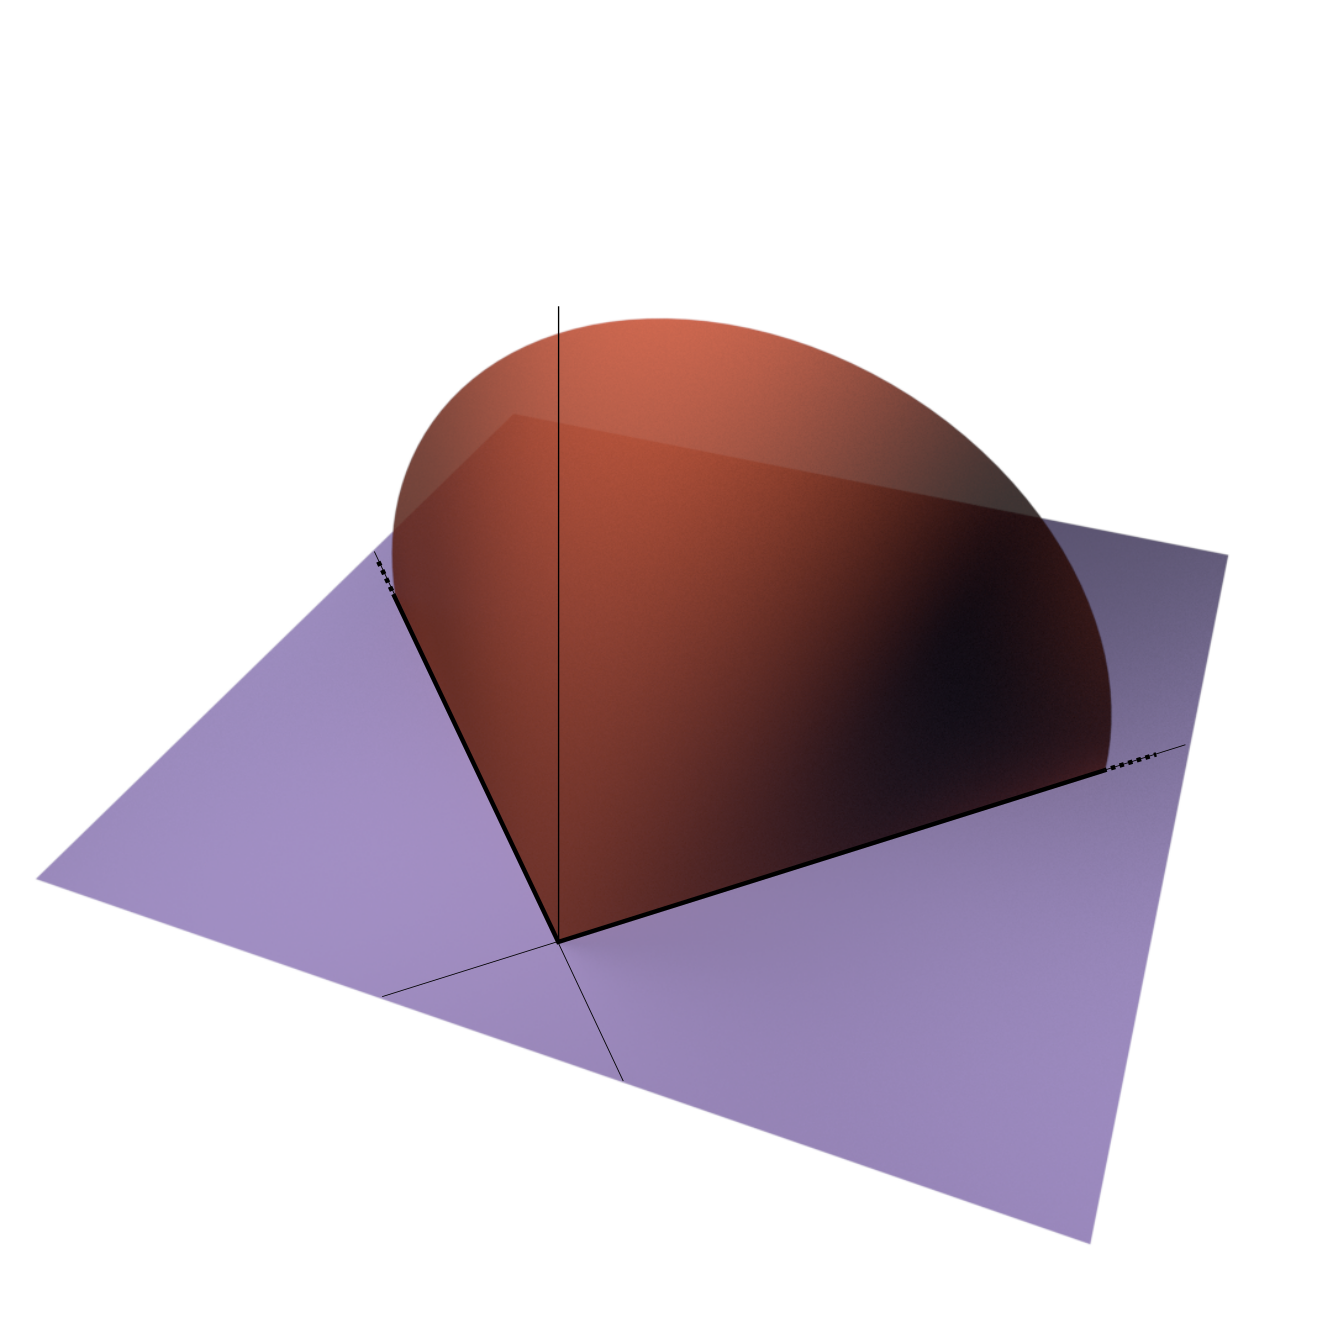
\includegraphics[width=0.7\textwidth]{cusp_worldsheet_vec.png}};
\begin{scope}[x={(image.south east)},y={(image.north west)}]
\node [anchor=west] at (0.32,0.35) {$\mathcal{C}$};
\node [anchor=west] at (0.63,0.75) {$\widetilde{\Sigma}$};
\node [anchor=west] at (0.39,0.8) {$z$};
\node [anchor=west] at (0.22,0.62) {$x^{+}$};
\node [anchor=west] at (0.9,0.45) {$x^{-}$};
%\draw[help lines,xstep=.1,ystep=.1] (0,0) grid (1,1);
%\foreach \x in {0,1,...,9} { \node [anchor=north] at (\x/10,0) {0.\x}; }
%\foreach \y in {0,1,...,9} { \node [anchor=east] at (0,\y/10) {0.\y}; }
\end{scope}
\end{tikzpicture}
\caption{Visualisation of the string worldsheet in the $AdS_{3}$ subspace (which is orthogonal to the coordinates $x,x^{*}$). For $z\to 0$ the embedding of the string worldsheet $\widetilde{\Sigma}$ is bounded by a cusped contour $\mathcal{C}$ closed at infinity.\label{fig: cusp_worldsheet}}
\end{center}
\end{figure}
%
%
For $z\to 0$ we approach the AdS boundary and therefore the regime of $\mathcal{N}=4$ SYM (see also \autoref{fig: cusp_worldsheet} for a visualization for the cusped contour). The curve proceeding at the boundary can be parametrised by
%
%
\begin{align}
\mathcal{C}_{\rm cusp}\quad :\quad (-\infty,\infty) \quad &\longrightarrow \quad \mathbb{R}^{4,1} \notag \\
%
s\qquad \; &\longrightarrow  \quad x^{1}=x^{2}=0, \\
&\qquad \quad x^{+}=\left\lbrace 
\begin{matrix}
-s\quad s<0, \\ 
0\quad {\rm else,}
\end{matrix} \right. \notag \\
&\qquad \quad x^{-}=\left\lbrace 
\begin{matrix}
\;\;\, s\quad s>0, \\ 
0\quad {\rm else.}
\end{matrix} \right. \notag
\end{align}
%
%
To arrive at the form of (\ref{eq: W_S_cusp}) with a fluctuation action $S_{\rm cusp}$, we need to expand $S_{\rm E}$ around the null-cusp background (\ref{eq: null_cusp}). We therefore choose the field fluctuations to be
%
%
\begin{equation}
x=\sqrt{\frac{\tau}{\sigma}}\tilde{x}, \quad z^{M}=\sqrt{\frac{\tau}{\sigma}}\tilde{z}^{M}, \quad \theta_{i}=\frac{1}{\sqrt{\sigma}}\tilde{\theta}_{i}, \quad \eta_{i} = \frac{1}{\sqrt{\sigma}}\tilde{\eta}_{i}.
\end{equation}
%
%
With a transition to the new worldsheet coordinates ${(\tau,\sigma)\to (t,s)=(\ln\tau , \ln \sigma)}$ the fluctuation action has no direct $t$ or $s$ dependence
%
%
\begin{align}
S_{\rm cusp} &= g \int \dd t \int \dd s \, \mathcal{L}_{\rm cusp} \label{eq: cusp_action} \\
%
%
\mathcal{L}_{\rm cusp} &= \left\vert \del_{t}\tilde{x} + \tfrac{1}{2}\tilde{x} \right\vert^{2} + \frac{1}{\tilde{z}^{4}}\left\vert \del_{s}\tilde{x} - \tfrac{1}{2}\tilde{x} \right\vert^{2} + \left( \del_{t}\tilde{z}^{M} + \frac{1}{2}\tilde{z}^{M} + \frac{i}{\tilde{z}^{2}}\tilde{z}_{N}\tilde{\eta}_{i} {\left(\rho^{MN}\right)^{i}}_{j} \tilde{\eta}^{j}\right)^{2} \notag \\
%
%
&\quad +\frac{1}{\tilde{z}^{4}}\left( \del_{s}\tilde{z}^{M} - \tfrac{1}{2} \tilde{z}^{M}\right)^{2} + i \left( \tilde{\theta}^{i}\del_{t}\tilde{\theta}_{i} + \tilde{\eta}^{i}\del_{t}\tilde{\eta}_{i} + \tilde{\theta}_{i}\del_{t}\tilde{\theta}^{i} + \tilde{\eta}_{i}\del_{t}\tilde{\eta}^{i}\right) - \frac{1}{\tilde{z}^{2}}\left(\tilde{\eta}^{2}\right)^{2} \notag \\
%
%
&\quad + \frac{2i}{\tilde{z}^{3}}\tilde{z}^{M}\tilde{\eta}^{i} \left(\rho^{M}\right)_{ij} \left( \del_{s}\tilde{\theta}^{j} - \frac{1}{2}\tilde{\theta}^{j} - \frac{i}{\tilde{z}} \tilde{\eta}^{j} \left(\del_{s}\tilde{x}- \tfrac{1}{2}\tilde{x}\right)\right) \notag \\
%
%
&\quad + \frac{2i}{\tilde{z}^{3}}\tilde{z}^{M}\tilde{\eta}_{i}\left(\rho_{M}^{\dagger}\right)^{ij} \left( \del_{s}\tilde{\theta}_{j} - \frac{1}{2} \tilde{\theta}_{j} + \frac{i}{\tilde{z}}\tilde{\eta}_{j} + \frac{i}{\tilde{z}} \tilde{\eta}^{j} \left(\del_{s}\tilde{x}- \tfrac{1}{2}\tilde{x}\right)^{*} \right). \notag
\end{align}
%
%
In the following we will drop the tilde notation for convenience. We also want to remark that there has been no truncation applied and this is still the full fluctuation action and therefore perfectly valid for a further application on non-perturbative calculations. In a previous step we set the light-cone momentum $p^{+}=1$ for simplicity, but since $p^{+}$ actually is a dimensionfull quantity we will insert a mass scale parameter $m$ that is also necessary for a later renormalization on the lattice and therefore change
%
%
\begin{align}
\del_{t}x +\frac{1}{2}x &\to \del_{t}x +\frac{m}{2}, & \del_{t}z^{M}+\frac{1}{2}z^{M} \to \del_{t}z^{M}+\frac{m}{2}z^{M}
\end{align}
%
%
and in the same way also the terms with spacial derivatives.
%
%
%
%
%
% - - - - - - - - -  Symmetries of the action - - - - - - - - - - - 
%
%
%
%
\subsection{Symmetries of the fluctuation action}
In \cite{Metsaev:2000yu} it was presented, that the general $\kappa$-symmetry light-cone fixed action possesses several symmetries. Two fundamental ones, which are also inherited by the fluctuation action (\ref{eq: cusp_action}) in its gauge fixed status, are global symmetries.
%
\begin{itemize}
\item At first a $U(1)\sim SO(2)$ symmetry which rotates the $x$ and $x^{*}$ coordinate fields orthogonal to the other $AdS_{5}$ coordinates, which therefore does not affect the classical solution. In order for the action to be invariant, also the fermions need to be shifted with the following transformations and the infinitesimal parameter $\epsilon$
%
%
\begin{equation}
\begin{alignedat}{9}
\delta x &= e^{i\epsilon}\; x, \qquad&  \delta\eta_{i}&= e^{i\frac{\epsilon}{2}}\; \eta_{i}, \qquad&  \delta\theta_{i} &= e^{-i\frac{\epsilon}{2}}\; \theta_{i},\\
\delta x^{*} &= e^{-i\epsilon}\; x^{*}, &  \delta\eta^{i}&= e^{-i\frac{\epsilon}{2}}\; \eta^{i}, &  \delta\theta^{i} &= e^{i\frac{\epsilon}{2}}\; \theta^{i}. 
\label{eq: U1_sym}
\end{alignedat}
\end{equation}
%
%
\item The other symmetry is an $SU(4)\sim SO(6)$, which concerns the $z^{M}$ fields and is inherited after gauge fixing due to the $S^{5}$ structure. By introducing an infinitesimal $SU(4)$ rotation ${\epsilon^{i}}_{j}$ the global symmetry transformations are given by
%
%
\begin{equation}
\begin{alignedat}{9}
\delta z^{M} &= -\frac{1}{2} {\epsilon^{i}}_{j} {(\rho^{MN})^{j}}_{i} z^{N}   \\
\delta \theta^{i} = {\epsilon^{i}}_{j} \theta ^{j}, \quad \delta \theta_{i} = -& \theta_{j} {\epsilon^{i}}_{j}, \quad  
\delta \eta ^{i} = {\epsilon^{i}}_{j} \eta^{i}, \quad  \delta \eta_{i}= - \eta_{i} {\epsilon^{i}}_{j}. 
\end{alignedat}
\end{equation}
%
%
Hereby one can see that the $z^{M}$ transform in the vector representation and the $\lbrace \eta^{i},\theta^{i}\rbrace$ and $\lbrace \eta_{i},\theta_{i}\rbrace$ in the fundamental and anti-fundamental representation of $SU(4)$, respectively.
\end{itemize}
%
%
%
%
% - - - - - - - - -   perturbative 1-loop free energy
%
%
%
%
%
\subsection{Perturbative 1-loop free energy}
Here we want to point out a quick check that fluctuations around the previously derived vacuum lead to the correct solution of (\ref{eq: scaling_fct}). We therefore want to reproduce the constant $\frac{3\ln 2}{\pi}$ term in $f(g)$. We know from (\ref{eq: W_exp_f}) that we can write
%
%
\begin{equation}
Z_{\rm string} = e^{-\frac{1}{8}f(\lambda)V_{2}} \equiv e^{-\Gamma(\lambda)}, \quad V_{2}=\int \dd t \int \dd s,
\end{equation}
%
%
where we define 
%
%
\begin{equation}
\Gamma = \Gamma^{(0)} + \Gamma^{(1)}+\Gamma^{(2)}+\cdots = \frac{1}{8}f(\lambda)V_{2}.
\end{equation}
%
%
Thereby $\Gamma^{(0)}=S_{\rm E}[X_{\rm cl},\mathit{\Psi}=0]$ is the value of the classical action on the solution and $\Gamma^{(1)},\Gamma^{(2)},\ldots$ are quantum corrections. The scaling function can be expanded in the following way
%
%
\begin{equation}
f(g) = g \left[ a_{0} + \frac{a_{1}}{g} + \frac{a_{2}}{g^{2}} + \cdots \right].
\end{equation}
%
%
In \cite{Giombi:2009gd} the 1-loop fluctuation coefficient $a_{1}$ has bee calculated via $\Gamma^{(1)}=-\ln Z^{(1)}$, where $Z^{(1)}$ is the exponential of the truncated fluctuation action that has only quadratic field contributions. The \names{Lagrangian} can therefore be written as a matrix-vector product with fermionic and bosonic matrix operators $\hat{D}_{\rm F}$ and $\hat{D}_{\rm B}$. The 1-loop approximation of the path integral can therefore be written as\footnote{With $\text{Det}\,\hat{O}$ we hereby mean the full infinite dimensional determinant in the sense of
\begin{equation*}
\ln \text{Det}\,\hat{O} = \text{Tr}\,\ln \hat{O} = \int \dd^{d}s \langle s\vert \text{tr}\,\ln\hat{O} \vert s \rangle
=\int \dd^{d}s \ln[\det O(s) ] ,
\end{equation*}
where tr and det refer to the regular trace and determinant if $\hat{O}$ is a matrix of operators and here $\vert s \rangle$ is an eigenbase of the operator $\hat{O}$.} (with $p^{2} = (p_{0})^{2}+(p_{1})^{2}$)
%
%
\begin{align}
\Gamma^{(1)} &= \frac{1}{2} \ln \frac{\text{Det}\, \hat{D}_{\rm B}}{\text{Det}\,\hat{D}_{\rm F}}
=  \frac{V_{2}}{2} \int \frac{\dd^{2}p}{(2\pi)^{2}} \; \ln \left[\frac{\det D_{\rm B}(p)}{\det D_{\rm F}(p)} \right]
\label{eq: 1_loop}      \\
%
%
&= \frac{V_{2}}{2} \int \frac{\dd^{2}p}{(2\pi)^{2}} \; \ln \left[ \frac{\left(p^{2} +m^{2}\right) \left( p^{2} +\frac{m^{2}}{2}\right)^{2} \left(p^{2}\right)^{5}}{\left( p^{2} + \frac{m^{2}}{4}\right)^{8}} \right]
=-\frac{3 \ln 2}{\pi} \frac{V_{2}}{8}m^{2},   \notag
\end{align}
%
%
leading to the correct 1-loop coefficient for $f(g)$ with $m=1$.